%TC: macro \marginfootnote [other]
%TC: envir SCfigure [] other
%TC: macrocount beginSCfigure [figure]
\documentclass[11pt,twoside]{report}
\usepackage{preamble}
\setcounter{chapter}{2}
\graphicspath{{../img/}}
\def\includebibliography{}
\renewcommand{\chaptername}{Appendix}
\renewcommand{\thechapter}{\Alph{chapter}}

\externaldocument{morphometric-applications}

\begin{document}
\chapter{Evaluating free energies of hard sphere structures analytically}
\label{appendix:bayesian}

This appendix describes analytical methods for evaluating the free energy of hard sphere structures used in chapter \ref{chapter:morphometric-applications} to obtain free energies along reaction paths.
We need to evaluate integrals of the form of \eqref{eq:schematic-partition-function} which we repeat here as
\begin{equation*}
  \mathcal{I}
  =
  \int_{D'}
  %e^{-\beta U_n(\vec{x})} \, y^{(n)}(\vec{x})
  g^{(n)}(\vec{x}) R(\vec{x})
  \, d^l \vec{x},
\end{equation*}
where $R(\vec{x})$ rotational metric.
In section \eqref{sec:analytic-integrals} we demonstrated that it is sufficient to solve
\begin{equation*}
  Z = \int_{\mathcal{D}'} g^{(n)}(\vec{x}) \, d^l \vec{x},
\end{equation*}
and to evaluate the effects of rotations perturbatively using \eqref{eq:rotation-metric-perturbations} it is sufficient to determine the first few moments of the probability distribution $p(\vec{x})$.
We restate its definition \eqref{eq:expanded-structure-p} as a reminder here as
\begin{equation*}
  \begin{split}
    p(\vec{x})
    &=
    \frac{y^{(n)}(\vec{x})}{Z}
    \,
    \prod_{(i,j) \in \mathcal{M}} \mathbb{I}_{[0, \delta]}(h_{ij})
    \prod_{\substack{i < j \\ (i,j) \notin \mathcal{M}}}
    \mathbb{I}_{[0, \infty]} (h_{ij}),
    %% \prod_{k = 1}^m \mathbb{I}_{[0, \delta]}(h_k)
    %% \prod_{\substack{i < j \\ (i,j) \notin \mathcal{M}}}
    %% \mathbb{I}_{[0, \infty]}(|\vec{r}_i - \vec{r}_j| - \sigma).
    \\ &\simeq
    \frac{y^{(n)}(\vec{x}^*) e^{-\vec{A} \cdot \Delta \vec{x}}}{Z}
    \,
    \prod_{(i,j) \in \mathcal{M}} \mathbb{I}_{[0, \delta]}(h_{ij})
    \prod_{\substack{i < j \\ (i,j) \notin \mathcal{M}}}
    \mathbb{I}_{[0, \infty]} (h_{ij}),
    %% \prod_{k = 1}^m \mathbb{I}_{[0, \delta]}(h_k)
    %% \prod_{\substack{i < j \\ (i,j) \notin \mathcal{M}}}
    %% \mathbb{I}_{[0, \infty]}(|\vec{r}_i - \vec{r}_j| - \sigma),
    %+ \mathcal{O}(\Delta \vec{x}^2)
  \end{split}
\end{equation*}
%% \begin{equation*}
%%   \begin{split}
%%   p(\vec{x})
%%   &=
%%   \frac{g^{(n)}(\vec{x}) \chi_{\mathcal{D}'}(\vec{x})}{Z}
%%   \\ &=
%%   \underbrace{
%%     \frac{y^{(n)}(\vec{x})}{Z}
%%     \vphantom{\prod_{i < j}}
%%   }_\textrm{smooth}
%%   \;
%%   \underbrace{
%%     \chi_{\mathcal{D}'}(\vec{x})
%%     \prod_{i < j}
%%     \Theta \Big( |\vec{r}_i - \vec{r}_j| - \sigma \Big)
%%   }_\textrm{singular terms},
%%   \\ &\simeq
%%   \frac{y^{(n)}(\vec{x}^*) e^{-\vec{A} \cdot \Delta \vec{x}}}{Z}
%%   \;
%%   \chi_{\mathcal{D}'}(\vec{x})
%%   \prod_{i < j}
%%   \Theta \Big( |\vec{r}_i - \vec{r}_j| - \sigma \Big)
%%   \end{split}
%% \end{equation*}
with $\int_{\mathbb{R}^l} p(\vec{x}) d^l\vec{x} = 1$, and in the final line we have used the first-order expansion of the potential of mean force \eqref{eq:cavity-perturbation} $\vec{A} = \nabla \beta\Omega(\vec{x}^*)$.
Introducing the \emph{tile distribution}
\begin{equation}\label{eq:ep-tile-distribution}
  t_{ij}(h_{ij})
  =
  \begin{cases}
    \mathbb{I}_{[0, \delta]}(h_{ij}) & \textrm{ if } (i,j) \in \mathcal{M} \\
    \mathbb{I}_{[0, \infty]}(h_{ij}) & \textrm{ if } (i,j) \notin \mathcal{M}
  \end{cases}
\end{equation}
then the probability distribution becomes
\begin{equation}\label{eq:ep-p-tiles}
  p(\vec{x})
  =
  \frac{y^{(n)}(\vec{x}^*) e^{-\vec{A} \cdot \Delta \vec{x}}}{Z}
  \,
  \prod_{i < j} t_{ij}(h_{ij}).
\end{equation}

Inspired by the Harmonic approximation \eqref{eq:harmonic-approximation}, where the energy is expanded to second order, we will attempt to approximate the basin probability distribution $p(\vec{x})$ as a Gaussian.
We write this approximate probability distribution as
\begin{equation}
  q(\vec{x}) = Z \mathcal{N}(\vec{x}; \vec{\mu}, \vec{\Sigma}).
\end{equation}
where we have kept it unnormalised for convenience (so it is not strictly a distribution) as our goal is to determine $Z$.
The moments of the Gaussian $\vec{\mu}, \vec{\Sigma}$ will be determined alongside $Z$, giving the evaluation of $I$ through \eqref{eq:rotation-metric-perturbations}.
%Note that in the Bayesian inference literature $p(\vec{x})$ would be called the posterior distribution.
Some relevant properties of multivariate Gaussians, including its explicit form, are given in section \ref{sec:gaussian-properties}

Consider the free energy difference between the true and approximate distribution
\begin{equation*}
  \Delta F
  =
  - \int p(\vec{x})
  \ln{\left( \frac{q(\vec{x})}{Z p(\vec{x})} \right)} \, d\vec{x}.
\end{equation*}
In information theory this would be called the \emph{Kullback-Leibler divergence}, a measure of information loss from using the approximate distribution $q(\vec{x})/Z$.
It is straightforward to prove that it is only zero when $p(\vec{x}) = q(\vec{x}) / Z$ \cite{MerminPR1965, EvansAP1979}, but this is impossible to achieve unless $p(\vec{x})$ is also Gaussian.
%It is schematically identical to the proof of the uniqueness of the equilibrium free energy.
However, by minimising $\Delta F$ we can optimise the parameters of $q(\vec{x})$ to minimise the error of the approximation.
It is straightforward to show that for distributions in the exponential family this corresponds to matching the moments of $q(\vec{x})$ and $p(\vec{x})$ \cite{Minka2001,MinkaUAI2001,Rasmussen2006,Cunningham2011}.
Matching the moments is still intractable because of the high dimensionality of $\vec{x}$.
Expectation propagation (EP) is a technique to approximate this procedure, which involves matching moments along marginal distributions instead of the whole space \cite{Minka2001,MinkaUAI2001,Rasmussen2006,Cunningham2011}.
This approximation scheme was inspired by the cavity method of spin glasses, for applications to approximate Bayesian inference.

In section \ref{sec:no-ep-integration} we show how $Z$ can be calculated exactly for the simplest case of minimally constrained geometries and where no additional hard sphere overlaps can occur over the integration domain; this approximation is valid for the smallest geometries up to $n \le 6$, however fails for $n=7$ where frustrated packings appear.
In subsequent sections we generalise this integration to the the more general case with additional hard sphere interactions using the approximation scheme outlined above.
In section \ref{sec:polyhedral-approximation} we introduce the \emph{polyhedral approximation} to the integration limits that simplifies treating the tile distributions appearing in \eqref{eq:ep-p-tiles}, before we describe the EP method to obtain the optimal Gaussian parameters in section \ref{sec:ep-integration}.
Throughout this exposition we invoke properties of multivariate Gaussians, which are summarised at the end in section \ref{sec:gaussian-properties}.
As this method is a little technical, we provide an example for a simple integration on a triangle in section \ref{sec:ep-worked-example} as an illustration.

%As discussed in section \ref{?} the minimum is not as thermodynamically significant as expected for soft systems because of the singularity of the hard sphere potential.

%% \section{Simple integral}

%% Finally, we write the distribution function in terms of the potential of mean force and expand this and the moment of inertia to first order, as in
%% \begin{align}
%%   \phi^{(n)}(\vec{x}) &=
%%   \phi^{(n)}(\vec{x}_0) +
%%   (\vec{x} - \vec{x}_0) \cdot
%%   \left. \vec{\nabla} \phi^{(n)}(\vec{x}) \right|_{\vec{x} = \vec{x}_0} +
%%   \mathcal{O}(\vec{x}^2), \\
%%   \sqrt{\det{\vec{I}(\vec{x})}} &=
%%   \sqrt{\det{\vec{I}(\vec{x}_0)}} +
%%   (\vec{x} - \vec{x}_0) \cdot
%%   \left. \vec{\nabla} \sqrt{\det{\vec{I}(\vec{x})}} \right|_{\vec{x} = \vec{x}_0} +
%%   \mathcal{O}(\vec{x}^2).
%% \end{align}
%% Using the analytical gradient expressions given in Section \ref{SI:line-curvature} makes this calculation very efficient.
%% The integral \eqref{eq:structural-partition-function-approximated} separates into $3n-6$ independent one-dimensional integrals of the form
%% \begin{equation*}
%%   \int_\sigma^{\sigma_{cut}} (a_i + b_i x_i) e^{-c_i x_i} dx_i
%%   = \left[
%%     - \left(
%%     \frac{(a + b_i x_i)}{c_i} + \frac{b_i}{c_i^2} \right) e^{-c_i x_i}
%%   \right]_\sigma^{\sigma_{cut}},
%% \end{equation*}
%% where $a_i$, $b_i$ and $c_i$ are constants.

%% Loosely speaking, this is the hard-particle analogue of the harmonic approximation with the difference here being that the first derivative does not vanish at the minimum.
%% For $n=6$ this expansion works rather well, as all structures have exactly $3n-6$ bonds and this perturbation theory captures the free energy well when compared with the ``exact'' result from thermodynamic integration.

\section{Minimally constrained geometries}
\label{sec:no-ep-integration}

First, we consider the simplest case of \emph{minimally constrained} geometries which have exactly $m = l$ bonds%
\marginfootnote{As a reminder, $l = 3n - 6$ is the number of (non-rigid body) degrees of freedom.},
so that the bond-distance space forms a natural basis for this expansion and we can set $\vec{x} = \{h_{a_1 b_1}, \cdots, h_{a_m b_m}\}$, with the energy minimum occurring at $\vec{x}^* = \{0, \cdots, 0\} = \vec{0}$.
This special case simplifies calculation in a similar way that isostaticity can be exploited to derive theories for systems approaching jamming, \cite{WyartAP2005,BritoEEL2006}.
However, we will have to consider the effects of additional hard sphere interactions and later using EP can generalise to the case where $m \ge l$.

As an aside, we describe how to calculate the internal metric entering into $R(\vec{x})$ for this choice of coordinates.
This metric is defined by
\begin{equation*}
  \overline{G_{ij}} = \vec{J}^T \vec{J}
\end{equation*}
where the Jacobian matrix entries are given by
\begin{equation*}
  J_{ij} = \frac{\partial x_i}{\partial h_{a_j b_j}}.
\end{equation*}
In practice it is usually easier to calculate its inverse numerically (via e.g.\ finite differences) using
\begin{equation*}
  J_{ij}^{-1} = \frac{\partial h_{a_i b_i}}{\partial x_j},
\end{equation*}
which has linearly independent rows for a minimally constrained geometry.
We can recover $\vec{J}$ from $\vec{K} := \vec{J}^{-1}$ using the matrix inversion formula $\vec{J} = (\vec{K}^T\vec{K})^{-1} \vec{K}^T$.

In this basis, the definition of structure (and limits of integration) is equivalent to a hypercube, i.e.\
\begin{equation*}
  \int_{D'} d^l x
  =
  \int_0^\delta dx_1 \cdots \int_0^\delta dx_m.
\end{equation*}
Helpfully, the hard sphere interactions between particle pairs $a_k,b_k \in \mathcal{M}$ have been absorbed into the integration limits, so we only have to consider the remaining $n(n-1)/2 - m$ interactions.
As our first approximation we ignore the effects of overlaps between any other particle pairs giving
\begin{subequations}
  \begin{align}
    Z
    &=
    \int_0^\delta dx_1 \cdots \int_0^\delta dx_m
    \, y^{(n)}(\vec{x})
    \\
    \langle \cdot \rangle_\mathcal{P}
    &=
    \frac{1}{Z}
    \int_0^\delta dx_1 \cdots \int_0^\delta dx_m
    \, (\cdot) y^{(n)}(\vec{x}).
  \end{align}
\end{subequations}
Introducing the perturbation expansion of the cavity function \eqref{eq:cavity-perturbation} we obtain
\begin{equation}
  \begin{split}
    Z
    &=
    y^{(n)}(\vec{x}^*)
    \prod_{i=1}^l
    \int_0^\delta
    \exp{\left( -\vec{A} \cdot \vec{e}_i \, x_i \right)}
    \, dx_i
    \\ &=
    y^{(n)}(\vec{x}^*)
    \prod_{i=1}^l
    \left[
    \frac{1 - \exp{\left( -A_i \, \delta \right)}}{A_i}
    \right]
  \end{split}
\end{equation}
with similar expressions for the first few moments.
Inserting this expression into the structural partition function \eqref{eq:structural-partition-function-detailed} yields expressions for the local structure's free energy/concentration.

The above formulae are rather simple, however the approximation is uncontrolled and we in general expect large errors for all but the most simple geometries: the hard sphere interactions should have a large effect.
We find that ignoring the effect of hard sphere interactions not in $\mathcal{M}$ to be a reasonably accurate approximation for $n \le 6$, however it fails for $n \ge 7$ with selected geometries.
In Fig.\ \ref{fig:ep-n7} (top panel) we see that the error in this method is comparable between 4 out of the 5 possible structures, with a similar trend against density.
However, one structure deviates strongly from the main trend with the error becoming substantial at high densities.
The geometry in question is a variant of the frustrated pentagonal bipyramid with broken fivefold symmetry (top variant Fig.\ \ref{fig:packings}); the particles with the broken bond are almost touching so ignoring their interaction is a serious approximation.
In general, we expect the majority of stable structures to require treatment of more hard sphere interactions than just the contacts.

To go beyond this approximation we will approximate the geometry of hard sphere interactions to leading order; in effect, this models the domain of integration as a polyhedron.
Finally, we will use the EP technique to evaluate the integral on the resulting polyhedron.

\section{Polyhedral approximation}
\label{sec:polyhedral-approximation}

The bond-distance arguments $h_{ij}$ to the tile distributions in \eqref{eq:ep-p-tiles} are complicated functions of $\vec{x}$ in general.
Our central simplifying approximation is to approximate them by an expansion to linear order, as in
\begin{equation*}
  h_{ij}(\vec{x})
  \simeq
  h_{ij}(\vec{x}^*)
  + \nabla h_{ij}(\vec{x}^*) \cdot \Delta \vec{x}
  + \mathcal{O}(\Delta \vec{x}^2),
\end{equation*}
To leading order, the tile distribution \eqref{eq:ep-tile-distribution} then constrains the bond distances to the regions
\begin{equation*}
  \nabla h_{ij}(\vec{x}^*) \cdot \Delta \vec{x}
  \in
  \begin{cases}
    [0, \delta] & \textrm{ if } (i,j) \in \mathcal{M} \\
    [-h_{ij}(\vec{x}^*), \infty] & \textrm{ if } (i,j) \notin \mathcal{M},
  \end{cases}
\end{equation*}
noting that $h_{ij}(\vec{x}^*) = 0$ iff $(i,j) \in \mathcal{M}$ by definition.
The latter line includes the $n(n-1)/2 - m$ interactions not covered by $\mathcal{M}$; empirically, for $n \le 7$ we find that most of these constraints are satisfied for all $\vec{x}$ (with $\delta \le 0.4\sigma$) and can be safely ignored.

Within this linear approximation, the combined effect of the tile distributions is to constrain the domain of integration to a high-dimensional polyhedron.
Our partition function becomes an integral of the cavity function, in the exponential family to leading order, over this polyhedron.
Similar approximations have been made for hard sphere free energy calculations in the crystal \cite{RadinPRL2005,KochPRE2005} and related systems \cite{LeoniPRL2017}; these approximations become exact at very high densities approaching close packing.

Finally, we note that for implementations the derivatives $\nabla h_{ij}$ have to be calculated in some coordinate basis.
For minimally constrained geometries with $m=l$ the natural basis is the bond-distances for pairs in $\mathcal{M}$ as outlined in the previous section.
For $m \ge l$ any choice of $m$ pairs will serve as a basis, though the choice may affect the end result.

\newpage
\section{Expectation propagation}
\label{sec:ep-integration}

Having introduced the relevant prerequisites, we now describe the EP algorithm which optimises the parameters of the approximate distribution $q(\vec{x})$ to obtain an estimate of the integral $Z$.
Our exposition of this technique closely follows \cite{Cunningham2011}.

%We start by noting that the true probability distribution, which includes the limits of integration, can be expressed as the product of distributions
For convenience we will ignore prefactors $y^{(n)}(\vec{x}^*)$ in \eqref{eq:ep-p-tiles}, which can be substituted back in at the end to obtain the full solution, and we assume in the chosen coordinates $\vec{x}^* = 0$ so that we can write $\Delta\vec{x} = \vec{x}$.
Then replacing the double indices in the tile distributions with a single index $h_{ij} \to h_k$ we have
\begin{equation*}
  p(\vec{x})
  =
  e^{-\vec{A} \cdot \vec{x}}
  \prod_{k=1}^{m^*} t_k (\vec{c}_k \cdot \vec{x})
\end{equation*}
where $\vec{c}_k = \nabla h_k(0)$ and $m^*$ is the number of tile distributions which contribute after making the polyhedral approximation of the previous section ($m \le m^* \le n(n-1)/2$).

The EP algorithm constructs projections in the marginal distributions parallel to each of these constraints.
The moments are then matched along these univariate distributions, which is much more tractable than for the full probability distribution.
To facilitate this, a natural decomposition of $q(\vec{x})$ involves writing it in terms of approximate tile distributions $\widetilde{t}_i$, i.e.\
\begin{equation}
  q(\vec{x})
  =
  e^{-\vec{A} \cdot \vec{x}} \,
  %p_0(\vec{x})
  \prod_{i=1}^{m^*} \widetilde{t}_i (x_i)
  =
  e^{-\vec{A} \cdot \vec{x}} \,
  %p_0(\vec{x})
  \prod_{i=1}^{m^*} \widetilde{Z}_i \mathcal{N}(x_i; \widetilde{\mu}_i, \widetilde{\sigma}_i^2)
\end{equation}
with projected values
\begin{subequations}
  \begin{align}
    x_i &= \vec{c}_i \cdot \vec{x} \\
    \mu_i &= \vec{c}_i \cdot \vec{\mu}
  \end{align}
\end{subequations}
for $i \in \{1,\cdots,m\}$.
From \eqref{eq:combined-normals} and \eqref{eq:biased-normal} we have
\begin{equation}
  \begin{split}
    q(\vec{x}) &=
    Z_0
    \exp{\left( -\vec{A} \cdot \vec{x} \right)} \,
    %p_0(\vec{x}) \,
    \mathcal{N}(\vec{x}; \vec{\Sigma} \cdot \vec{\nu}, \vec{\Sigma}) \\
    &=
    Z_0
    \exp{\left( \frac{\vec{A} \cdot \vec{\Sigma} \cdot \vec{A}}{2} - \vec{A} \cdot \vec{\Sigma} \cdot{\vec{\nu}} \right)} \,
    \mathcal{N}(\vec{x}; \vec{\Sigma} \cdot (\vec{\nu} - \vec{A}), \vec{\Sigma})
  \end{split}
\end{equation}
where $\vec{\Sigma}, \vec{\nu}, Z_0$ are given by \eqref{eq:combined-normals-sigma}, \eqref{eq:combined-normals-nu} and \eqref{eq:combined-normals-Z} respectively.
We thus have
\begin{subequations}
  \begin{align}
    \vec{\mu} &= \vec{\Sigma} \cdot (\vec{\nu} - \vec{A})
    \\
    Z &= Z_0
    \exp{\left( \frac{\vec{A} \cdot \vec{\Sigma} \cdot \vec{A}}{2} - \vec{A} \cdot \vec{\Sigma} \cdot \vec{\nu} \right)}
    \\
    Z_0 &=
    \sqrt{ (2\pi)^{l-m^*} \det{\vec{\Sigma}} }
    \;
    \exp{\left( \frac{\vec{\nu} \cdot \vec{\Sigma} \cdot \vec{\nu}}{2} \right)}
    \prod_{i=1}^{m^*}
    \left(
    \frac{\widetilde{Z}_i}{\sqrt{ \widetilde{\sigma}_i^2 }}
    \exp{\left(-\frac{\widetilde{\nu}_i \widetilde{\mu}_i}{2}\right)}
    \right)
  \end{align}
\end{subequations}
We marginalise the full probability distribution along one direction to obtain the cavity distribution
\begin{equation}
  q^{\setminus i}(\vec{x}) =
  \frac{\widetilde{Z}_i}{Z} \frac{q(\vec{x})}{\widetilde{t}_i(x_i)}
  =
  \frac
      {\mathcal{N}(\vec{x}; \vec{\mu}, \vec{\Sigma})}
      {\mathcal{N}(x_i; \widetilde{\mu}_i, \widetilde{\sigma}_i^2)}.
\end{equation}
This particular normalisation is chosen such that
\begin{equation}\label{eq:approximate-zeroth-moment}
  \int_{\mathbb{R}^l} q^{\setminus i}(\vec{x}) \widetilde{t}_i(x_i) \, d\vec{x} =
  \widetilde{Z}_i \int_{\mathbb{R}^l} \mathcal{N}(\vec{x}; \vec{\mu}, \vec{\Sigma}) \, d\vec{x} =
  \widetilde{Z}_i.
\end{equation}
Integrating this cavity over the orthogonal affine space gives
\begin{equation}
  \begin{split}
    q_{\setminus i}(x_i) :=&
    \int_{\mathbb{R}^l \setminus \vec{c}_i} q^{\setminus i} (\vec{x}_{\setminus i}; x_i) \, d\vec{x}_{\setminus i} \\
    =& \frac{1}{\mathcal{N}(x_i; \widetilde{\mu}_i, \widetilde{\sigma}_i^2)}
    \int_{\mathbb{R}^l \setminus \vec{c}_i} \mathcal{N}(\vec{x}; \vec{\mu}, \vec{\Sigma}) \, d\vec{x}_{\setminus i} \\
    =&
    \frac
        {\mathcal{N}(x_i; \mu_i, \vec{c}_i \cdot \vec{\Sigma} \cdot \vec{c}_i)}
        {\mathcal{N}(x_i; \widetilde{\mu}_i, \widetilde{\sigma}_i^2)} \\
    =&
        \sqrt{ \frac{\widetilde{\sigma}_i^2}{\vec{c}_i \cdot \vec{\Sigma} \cdot \vec{c}_i} }
        \exp{\left( -\frac{(x_i - \mu_i)^2}{2 \vec{c}_i \cdot \vec{\Sigma} \cdot \vec{c}_i} +
          \frac{(x_i - \widetilde{\mu}_i)^2}{2 \widetilde{\sigma}_i^2} \right)} \\
    =&
        \sqrt{ \frac{\sigma_{\setminus i}^2 + \widetilde{\sigma}_i^2}{\sigma_{\setminus i}^2} }
        \exp{\left(
          - \frac{(x_i - \mu_{\setminus i})^2}{2 \sigma_{\setminus i}^2}
          + \frac{1}{2}
          \frac{(\mu_{\setminus i} - \widetilde{\mu}_i)^2}{\sigma_{\setminus i}^2 + \widetilde{\sigma}_i^2}
          \right)} \\
     =& Z_{\setminus i} \, \mathcal{N}(x_i; \mu_{\setminus i}, \sigma_{\setminus i}^2)
  \end{split}
\end{equation}
where we completed the square in the penultimate step using the cavity parameters: \cite{Rasmussen2006,Cunningham2011}
\begin{align}
  Z_{\setminus i}
  &=
  \sqrt{2 \pi (\sigma_{\setminus i}^2 + \widetilde{\sigma}_i^2)}
  \exp{\left(
    \frac{1}{2}
    \frac{(\mu_{\setminus i} - \widetilde{\mu}_i)^2}{\sigma_{\setminus i}^2 + \widetilde{\sigma}_i^2}
    \right)}
        \\
  \sigma_{\setminus i}^2 &= \left(
  \frac{1}{\vec{c}_i \cdot \vec{\Sigma} \cdot \vec{c}_i} - \frac{1}{\widetilde{\sigma}_i^2}
  \right)^{-1} \\
  \mu_{\setminus i} &= \sigma_{\setminus i}^2 \left(
  \frac{\mu_i}{\vec{c}_i \cdot \vec{\Sigma} \cdot \vec{c}_i} - \frac{\widetilde{\mu}_i}{\widetilde{\sigma}_i^2}
  \right).
\end{align}
Note that the cavity distribution is the properly normalised quantity $q_{\setminus i}(x_i) / Z_{\setminus i}$.
The exact zeroth cavity moment is found via \cite{Cunningham2011}
\begin{equation}\label{eq:exact-zeroth-moment}
  \begin{split}
    \frac{\widehat{Z}_i}{Z_{\setminus i}}
    &=
    \frac{1}{Z_{\setminus i}}
    \int_{\mathbb{R}} q_{\setminus i}(x_i) t_i(x_i) \, dx_i
    \\ &=
    \frac{1}{Z_{\setminus i}}
    \int_{l_i}^{u_i} q_{\setminus i}(x_i) \, dx_i
    =
    \frac{1}{2} \left( \erf{\beta_i} - \erf{\alpha_i} \right)
  \end{split}
\end{equation}
where $l_i, u_i$ are the limits imposed by the tile distribution, and where we have introduced the shorthand
\begin{align}
  \alpha_i &= \frac{l_i - \mu_{\setminus i}}{\sqrt{2} \sigma_{\setminus i}} \\
  \beta_i &= \frac{u_i - \mu_{\setminus i}}{\sqrt{2} \sigma_{\setminus i}}.
\end{align}
The above relations are numerically unstable in the limit of small $\sigma_i^2 - \widetilde{\sigma}_i^2$, so we have to handle this case by Taylor expansion:
\begin{align}
  q_{\setminus i}(x_i) &=
  \frac{
    \mathcal{N}(x_i; \vec{c}_i \cdot \vec{\mu}, \vec{c}_i \cdot \vec{\Sigma} \cdot \vec{c}_i)
  }{
    \mathcal{N}(x_i; \widetilde{\mu}_i, \widetilde{\sigma}_i^2)
  }
  =
  \frac{\mathcal{N}(x_i; \mu_i, \sigma_i^2)}{
    \mathcal{N}(x_i; \widetilde{\mu}_i, \widetilde{\sigma}_i^2)
  }
  \nonumber \\ &=
  \exp{\left(-A_i x_i
    - \frac{A_i^2 \sigma_i^2}{2}
    + A_i \mu_i
    \right)}
  \frac{\mathcal{N}(x_i; \mu_i + A_i \sigma_i^2, \sigma_i^2)}{
    \mathcal{N}(x_i; \widetilde{\mu}_i, \widetilde{\sigma}_i^2)
  }
\end{align}
where $A_i = \vec{A} \cdot \vec{c}_i$, giving
\begin{align}
  \widehat{Z}_i
  =&
  \int_{\mathbb{R}} q_{\setminus i}(x_i) t_i(x_i) \, dx_i
  \nonumber \\ =&
  \sqrt{ \frac{\widetilde{\sigma}_i^2}{\vec{c}_i \cdot \vec{\Sigma} \cdot \vec{c}_i} }
  %\int_0^{\delta_i}
  \int_{l_i}^{u_i}
  \exp{\left( -\frac{(x_i - \mu_i)^2}{2 \vec{c}_i \cdot \vec{\Sigma} \cdot \vec{c}_i} +
    \frac{(x_i - \widetilde{\mu}_i)^2}{2 \widetilde{\sigma}_i^2} \right)}
  %t_i(x_i)
  \, dx_i,
  %% \nonumber \\ =&
  %% \sqrt{ \frac{\widetilde{\sigma}_i^2}{\vec{c}_i \cdot \vec{\Sigma} \cdot \vec{c}_i} }
  %% \exp{\left(
  %%   - \frac{A_i^2 \sigma_i^2}{2}
  %%   + A_i \mu_i
  %%   \right)}
  %% \nonumber \\ &
  %% \times \int_0^{\delta_i}
  %% \exp{\left( -\frac{(x_i - (\mu_i + A_i \sigma_i^2))^2}{2 \vec{c}_i \cdot \vec{\Sigma} \cdot \vec{c}_i} +
  %%   \frac{(x_i - \widetilde{\mu}_i)^2}{2 \widetilde{\sigma}_i^2} - A_i x_i \right)} \, dx_i.
\end{align}
which is in a suitable form for a perturbation expansion.

In the EP algorithm an iterative scheme is constructed to obtain the parameters $\{\widetilde{Z}_i, \widetilde{\mu}_i, \widetilde{\sigma}_i^2\}$ so that the equality \eqref{eq:exact-zeroth-moment} is achieved along with similar equalities for the higher-order moments \cite{Minka2001,MinkaUAI2001,Rasmussen2006,Cunningham2011}.
This process is simpler than before because in each iteration the parameters are univariate.
After obtaining the optimal parameters, we have to the univariate distributions back together to obtain the final value of $Z$.
Matching moments between \eqref{eq:approximate-zeroth-moment} and \eqref{eq:exact-zeroth-moment} gives us
\begin{equation}
  \widetilde{Z}_i = \frac{\widehat{Z}_i}{Z_{\setminus i}}
  \sqrt{2 \pi (\sigma_{\setminus i}^2 + \widetilde{\sigma}_i^2)}
  \exp{\left(
    \frac{1}{2}
    \frac{(\mu_{\setminus i} - \widetilde{\mu}_i)^2}{\sigma_{\setminus i}^2 + \widetilde{\sigma}_i^2}
    \right)}.
\end{equation}
We calculate $\widehat{Z}_i / Z_{\setminus i}$ from \eqref{eq:exact-zeroth-moment} and then obtain the partition function as
\begin{equation}\label{eq:well-behaved-logZhat}
  \begin{split}
    \log{\widetilde{Z}_i}
    =
    \frac{1}{2} \left(
    \log{(2\pi)} +
    \log{(\sigma_{\setminus i}^2 + \widetilde{\sigma}_i^2)} +
    \frac{(\mu_{\setminus i} - \widetilde{\mu}_i)^2}{\sigma_{\setminus i}^2 + \widetilde{\sigma}_i^2}
    \right.&
    \\
    \left.
    + \log{\left(\frac{\erf{\beta_i} - \erf{\alpha_i}}{2}\right)}
    \right)&.
  \end{split}
\end{equation}
From \eqref{eq:pre-ep-logZ} the final partition function is found as
\begin{equation}
  \begin{split}
    \log{Z}
    =&
    \frac{1}{2} \Big(
    (l-m^*) \log{2\pi}
    + \log\det{\vec{\Sigma}}
    + \vec{\nu} \cdot \vec{\Sigma} \cdot \vec{\nu}
    \Big)
    \\ &
    + \sum_{i=1}^{m^*} \left(
    \log{\widetilde{Z}_i}
    - \frac{1}{2}
    \left(
    \log{\widetilde{\sigma}_i^2}
    %+ \widetilde{\nu}_i \widetilde{\mu}_i
    + \frac{\widetilde{\mu}_i^2}{\widetilde{\sigma}_i^2}
    \right)
    \right)
  \end{split}
\end{equation}
where the term inside the summation is given by \cite{Cunningham2011}
\begin{align}
  & \log{\widetilde{Z}_i}
  - \frac{1}{2}
  \left(
  \log{\widetilde{\sigma}_i^2}
  + \frac{\widetilde{\mu}_i^2}{\widetilde{\sigma}_i^2}
  \right)
  %% \nonumber \\ =&
  %% \frac{1}{2} \left(
  %% \log{(2\pi)} +
  %% \log{(\sigma_{\setminus i}^2 + \widetilde{\sigma}_i^2)} +
  %% \frac{(\mu_{\setminus i} - \widetilde{\mu}_i)^2}{\sigma_{\setminus i}^2 + \widetilde{\sigma}_i^2}
  %% \right.
  %% \nonumber \\ & \qquad
  %% \left.
  %% + \log{\left(\frac{\erf{\beta_i} - \erf{\alpha_i}}{2}\right)}
  %% - \log{\widetilde{\sigma}_i^2}
  %% - \widetilde{\nu}_i \widetilde{\mu}_i
  %% \right)
  \nonumber \\ =&
  \frac{1}{2} \left(
  \log{(2\pi)} +
  \log{\left(\frac{\sigma_{\setminus i}^2 + \widetilde{\sigma}_i^2}{\widetilde{\sigma}_i^2}\right)}
  + \frac{(\mu_{\setminus i} - \widetilde{\mu}_i)^2}{\sigma_{\setminus i}^2 + \widetilde{\sigma}_i^2}
  \right.
  \nonumber \\ & \qquad
  \left.
  %- \widetilde{\nu}_i \widetilde{\mu}_i
  - \frac{\widetilde{\mu}_i^2}{\widetilde{\sigma}_i^2}
  + \log{\left(\frac{\erf{\beta_i} - \erf{\alpha_i}}{2}\right)}
  \right),
  %% \nonumber \\ =&
  %% \frac{1}{2} \left(
  %% \log{(2\pi)} +
  %% \log{(1 + \widetilde{\tau}_i \sigma_{\setminus i}^2)}
  %% + \frac{\widetilde{\tau}_i \mu_{\setminus i}^2 - 2\widetilde{\nu}_i \mu_{\setminus i} - \widetilde{\nu}_i^2 \sigma_{\setminus i}^2}
  %% {1 + \widetilde{\tau}_i \sigma_{\setminus i}^2}
  %% \right.
  %% \nonumber \\ & \qquad
  %% \left.
  %% + \log{\left(\frac{\erf{\beta_i} - \erf{\alpha_i}}{2}\right)}
  %% \right),
\end{align}
from \eqref{eq:well-behaved-logZhat}.
Note that the latter quantity is numerically unstable for small $\sigma_i^2 - \widetilde{\sigma}_i^2$, so a perturbation expansion must be used instead; this ensures that this method reduces to the exact integral of section \ref{sec:no-ep-integration} in cases where $m=l$ and no additional hard sphere overlaps are possible.

In Fig.\ \ref{fig:ep-n7} (bottom panel) we see that this method can handle the effect of additional hard sphere interactions.
There is a systematic error brought about by the approximations in this integration scheme, however this error scales similarly for all 5 of the packings available for $n=7$ particles.

This has been a rather technical account of the method, so in the next section we show how $q(\vec{x})$ approximates the tile distributions in the simple case of an integration over a triangle.

\begin{SCfigure}
  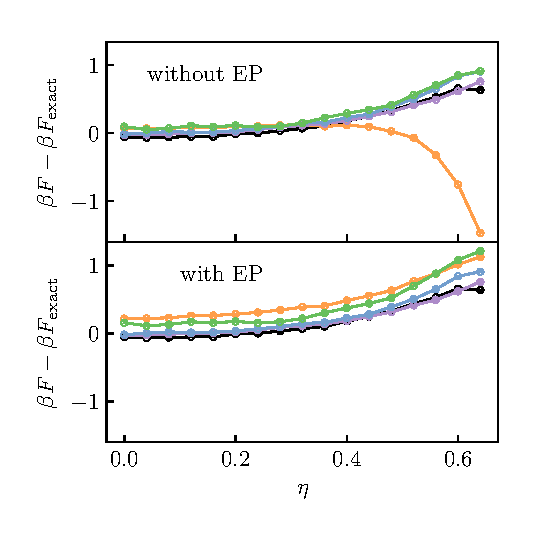
\includegraphics[width=0.9\linewidth,outer]{ep-n7}
  \caption[Errors in analytical integration techniques for the free energies of $n=7$ structures]{
    Errors in analytic integration techniques for free energies of the five $n = 7$ structures in Fig.\ \ref{fig:packings}.
    Top panel: simple integration ignoring hard sphere interactions not explicitly captured by the boundary conditions (section \ref{sec:no-ep-integration}).
    Bottom panel: expectation propagation (EP) integration which approximates the combined effect of boundary conditions and hard sphere interactions using (section \ref{sec:ep-integration}).
    In each case, the numerically exact result was obtained using thermodynamic integration described in chapter \ref{chapter:morphometric-applications}.
    The orange curve which deviates from the main trend without EP is the structure corresponding to a pentagonal bipyramid with broken fivefold symmetry; treatment of the broken bond with EP corrects the deviation.
  }
  \label{fig:ep-n7}
\end{SCfigure}

\section{Worked example: area of a triangle}
\label{sec:ep-worked-example}

As a simple worked example we consider the area of a right-angled triangle with vertices $(0,0)$, $(1,0)$, and $(0,1)$ i.e.\ half of the unit square.
We can write this area as the integral over a box
\begin{equation}\label{eq:ep-area-integral}
  A_\Delta = \int_0^1 \int_0^1 \Theta(1 - x - y) \, dx dy
  = \frac{1}{2}
\end{equation}
where $\Theta(\cdot)$ is the Heaviside function.
The exact result is fairly trivial, but it has the same form as the integrals we have been studying with e.g.\ $x,y$ representing the contact particles and $\Theta(1 - x - y)$ representing an additional hard sphere interaction between non-contact particles.
As such, we can evaluate the area using expectation propagation giving $A_\Delta^\mathrm{EP} \simeq 0.515$ for an error of about 3\%.
The effective probability distribution $p(x,y)$ for this integral is shown in \ref{fig:ep-pdf} (lower panel) which illustrates how the method builds in geometric information of additional constraints (in this case $\Theta(1 - x - y)$.
The distribution for the equivalent integral without this constraint is shown in the same figure (upper panel).

As an extension of the above problem we introduce an external field representing the perturbation expansion of the potential of mean force $\phi^{(n)}$.
We obtain the integral
\begin{equation}\label{eq:ep-triangle-integral}
  Z_\Delta = \int_0^1 \int_0^1 \Theta(1 - x - y) e^{-A_x x  A_y y} \, dx dy
\end{equation}
with the errors of expectation propagation shown in Fig.\ \ref{fig:ep-errors}.
The error of 3\% in the area is recovered in the limit $\vec{A} \to 0$, which increases to a maximum of around 4\% at moderate field strength.
At very large field strengths the error drops to essentially zero as the effect of the extra boundary condition is not seen, and the method becomes exact.


\begin{SCfigure}
  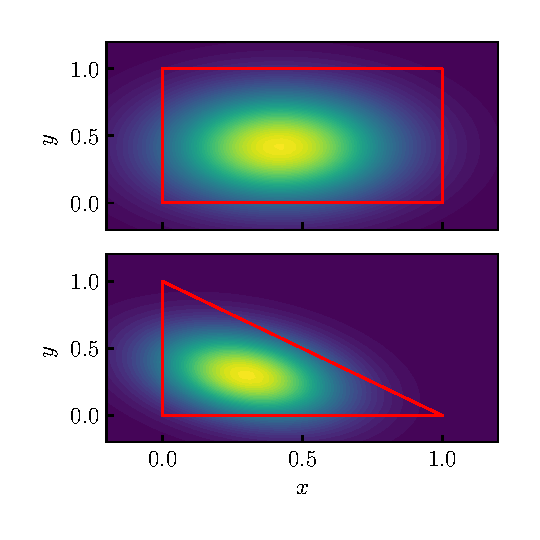
\includegraphics[width=0.9\linewidth,outer]{ep-pdf}
  \caption[Approximate probability distribution for integrating areas of simple 2d shapes]{
    Approximate (Gaussian) probability distribution $q(x,y)$ produced by expectation propagation for an integration over a square (top) and a right-angled triangle (bottom).
    In each panel the boundary of the true integration area is indicated by red lines, though the approximate probability distribution spans all of space.
  }
  \label{fig:ep-pdf}
\end{SCfigure}

\section{Addendum: properties of multivariate Gaussians}
\label{sec:gaussian-properties}

The multivariate Gaussian is defined as
\begin{equation}
  \begin{split}
    \mathcal{N}(\vec{x}; \vec{\mu}, \vec{\Sigma})
    :=&
    \frac{1}{\sqrt{ (2\pi)^l \det{\vec{\Sigma}} }}
    \exp{\left(
      - \frac{1}{2} (\vec{x} - \vec{\mu}) \cdot \vec{\Sigma}^{-1} \cdot (\vec{x} - \vec{\mu})
      \right)}
    \\
    =&
    \frac{1}{\sqrt{ (2\pi)^l \det{\vec{\Sigma}} }}
    \exp{\left(
      - \frac{\vec{x} \cdot \vec{\Sigma}^{-1} \cdot \vec{x}}{2}
      + \vec{x} \cdot \vec{\Sigma}^{-1} \cdot \vec{\mu}
      - \frac{\vec{\mu} \cdot \vec{\Sigma}^{-1} \cdot \vec{\mu}}{2}
      \right)}
  \end{split}
\end{equation}
where $\vec{x} \in \mathbb{R}^l$ is the Gaussian distributed vector in our phase space, with mean $\vec{\mu} \in \mathbb{R}^l$ and (positive-definite) covariance matrix $\vec{\Sigma} \in \mathbb{R}^{l \times l}$.

\begin{SCfigure}
  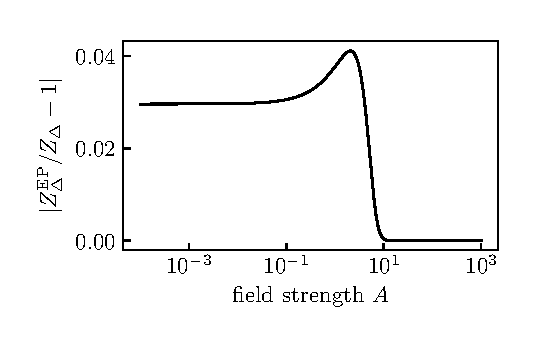
\includegraphics[width=0.9\linewidth,outer]{ep-errors}
  \caption[Errors in expectation propagation for integrating a field over a triangle]{
    Errors in expectation propagation for integrating a field over a triangle.
    The exact integral is given by \eqref{eq:ep-triangle-integral}, taking field $\vec{A} = (A, A)$.
  }
  \label{fig:ep-errors}
\end{SCfigure}

In the EP algorithm we wrote the multivariate Gaussian approximation in $q$ as the product of univariate Gaussians from the tile distributions approximating the boundary conditions.
To show this, consider the product of univariate Gaussians:
\begin{align}
  %\begin{split}
    &
    \prod_{i=1}^{m^*}
    \mathcal{N}(\vec{c}_i \cdot \vec{x}; \widetilde{\mu}_i, \widetilde{\sigma}_i^2)
    %\nonumber \\ =&
    =
    \prod_{i=1}^{m^*}
    \left(
    \frac{1}{\sqrt{ 2\pi \widetilde{\sigma}_i^2 }}
    \exp{\left(
      - \frac{1}{2} \frac{(\vec{c}_i \cdot \vec{x} - \widetilde{\mu}_i)^2}{\widetilde{\sigma}_i^2}
      \right)}
    \right)
    %% \nonumber \\ =&
    %% \prod_{i=1}^{m^*}
    %% \left(
    %% \frac{1}{\sqrt{ 2\pi \widetilde{\sigma}_i^2 }}
    %% \exp{\left(
    %%   - \frac{(\vec{c}_i \cdot \vec{x})^2}{2\widetilde{\sigma}_i^2}
    %%   + \frac{\widetilde{\mu}_i(\vec{c}_i \cdot \vec{x})}{\widetilde{\sigma}_i^2}
    %%   - \frac{\widetilde{\mu}_i^2}{2\widetilde{\sigma}_i^2}
    %%   \right)}
    %% \right)
    \nonumber \\ =&
    \prod_{i=1}^{m^*}
    \left(
    \frac{1}{\sqrt{ 2\pi \widetilde{\sigma}_i^2 }}
    \exp{\left(-\frac{\widetilde{\mu}_i^2}{2\widetilde{\sigma}_i^2}\right)}
    \right)
    \exp{\left( \sum_{i=1}^{m^*} \left(
      - \frac{(\vec{c}_i \cdot \vec{x})^2}{2\widetilde{\sigma}_i^2}
      + \frac{\widetilde{\mu}_i(\vec{c}_i \cdot \vec{x})}{\widetilde{\sigma}_i^2}
      \right) \right)}
    %% \nonumber \\ =&
    %% \prod_{i=1}^{m^*}
    %% \left(
    %% \frac{1}{\sqrt{ 2\pi \widetilde{\sigma}_i^2 }}
    %% \exp{\left(-\frac{\widetilde{\nu}_i \widetilde{\mu}_i}{2}\right)}
    %% \right)
    %% \exp{\left( \sum_{i=1}^{m^*} \left(
    %%   - \vec{x} \cdot \frac{\vec{c}_i \otimes \vec{c}_i}{2\widetilde{\sigma}_i^2} \cdot \vec{x}
    %%   + (\widetilde{\nu}_i\vec{c}_i) \cdot \vec{x}
    %%   \right) \right)}
    %% \nonumber \\ =&
    %% \prod_{i=1}^{m^*}
    %% \left(
    %% \frac{1}{\sqrt{ 2\pi \widetilde{\sigma}_i^2 }}
    %% \exp{\left(-\frac{\widetilde{\nu}_i \widetilde{\mu}_i}{2}\right)}
    %% \right)
    %% \mathcal{N}(\vec{x}; \vec{\mu}, \Sigma)
    %% \;
    %% \sqrt{ (2\pi)^l \det{\vec{\Sigma}} }
    %% \;
    %% \exp{\left( \frac{\vec{\mu} \cdot \vec{\Sigma}^{-1} \cdot \vec{\mu}}{2} \right)}
    \nonumber \\ =&
    \prod_{i=1}^{m^*}
    \left(
    \frac{1}{\sqrt{ 2\pi \widetilde{\sigma}_i^2 }}
    \exp{\left(-\frac{\widetilde{\nu}_i \widetilde{\mu}_i}{2}\right)}
    \right)
    \mathcal{N}(\vec{x}; \vec{\mu}, \Sigma)
    \;
    \sqrt{ (2\pi)^l \det{\vec{\Sigma}} }
    \;
    \exp{\left( \frac{\vec{\nu} \cdot \vec{\Sigma} \cdot \vec{\nu}}{2} \right)}
    \nonumber \\ =&
    Z \mathcal{N}(\vec{x}; \vec{\mu}, \Sigma)
  %\end{split}
  \label{eq:combined-normals}
\end{align}
with
\begin{subequations}
\begin{align}
  \widetilde{\nu}_i &= \frac{\widetilde{\mu}_i}{\widetilde{\sigma}_i^2} \\
  \vec{\Sigma}^{-1} &= \sum_{i=1}^{m^*} \frac{\vec{c}_i \otimes \vec{c}_i}{\widetilde{\sigma}_i^2}
  \label{eq:combined-normals-sigma}
  \\
  \vec{\mu} &=
  \vec{\Sigma} \cdot \left( \sum_{i=1}^{m^*} \widetilde{\nu}_i \vec{c}_i \right)
  = \vec{\Sigma} \cdot \vec{\nu}
  \\
  \vec{\nu} &= \sum_{i=1}^{m^*} \widetilde{\nu}_i \vec{c}_i
  \label{eq:combined-normals-nu}
  \\
  Z &=
  \sqrt{ (2\pi)^{l-m^*} \det{\vec{\Sigma}} }
  \;
  \exp{\left( \frac{\vec{\nu} \cdot \vec{\Sigma} \cdot \vec{\nu}}{2} \right)}
  \prod_{i=1}^{m^*}
  %\left(
  \frac{1}{\sqrt{ \widetilde{\sigma}_i^2 }}
  \exp{\left(-\frac{\widetilde{\nu}_i \widetilde{\mu}_i}{2}\right)}
  %\right)
  \label{eq:combined-normals-Z}
\end{align}
\end{subequations}
From this we find that
\begin{equation}\label{eq:pre-ep-logZ}
  \log{Z} =
  \frac{l-m^*}{2} \log{2\pi} +
  \frac{1}{2} \log\det{\vec{\Sigma}} +
  \frac{\vec{\nu} \cdot \vec{\Sigma} \cdot \vec{\nu}}{2} -
  \sum_{i=1}^{m^*}
  \left(
  \frac{1}{2} \log{\widetilde{\sigma}_i^2} +
  \frac{\widetilde{\nu}_i \widetilde{\mu}_i}{2}
  \right)
\end{equation}
Finally, note that
\begin{equation}\label{eq:biased-normal}
  e^{-\vec{A} \cdot \vec{x}} \mathcal{N}(\vec{x}; \vec{\mu}, \vec{\Sigma})
  =
  \exp{\left( \frac{\vec{A} \cdot \vec{\Sigma} \cdot \vec{A}}{2} - \vec{A} \cdot \vec{\mu} \right)} \;
  \mathcal{N}(\vec{x}; \vec{\mu} - \vec{\Sigma}\cdot\vec{A}, \vec{\Sigma}).
\end{equation}

\ifdefined\includebibliography
  \newgeometry{margin=1in}
  \printbibliography
\fi

\end{document}
